
\chapter{基于反卷积神经网络的二维人体姿态估计}

\section{基于深度学习的二维人体姿态估计}
二维人体姿态估计任务,需要从原始图像或视频中,识别和定位人体骨架关节点并估计其二维坐标。

二维人体姿态估计具有如下难点:

\begin{enumerate}
    \item 遮挡和自遮挡。在复杂环境下和多人图像中,目标人体的部位难以避免地被前景、他人和自身部位及衣着遮挡,故而产生难以检测的关节点。
    \item 复杂的前景背景。除了遮挡之外,在多人姿态估计中,相邻目标人体的相似部位易导致区分和还原每个目标的正确姿态时发生混淆。
    \item 多样的人体姿态。除了人体的常见动作,如由走、坐构成的日常行为外,在极端的场景和特殊的相机视角下,会出现很多罕见的二维姿态投影,而难以被数据集覆盖。

\end{enumerate}

故而在对RGB图像进行关节坐标的预测时,对关节点进行精确的识别和坐标预测需要局部的细节信息,同时估计整个人体合理的姿态又需要对全局信息有正确的把握,以获取如人物朝向,肢体方位关系等信息。故而在网络架构中,进行下采样后,再上采样生成高分辨率特征图成为了网络设计的关键技术。

针对如上问题,2016年,Newell等提出了一个二维人体姿态估计模型\textsuperscript{\cite{p23}},用一种新颖的堆叠沙漏网络(Stacked Hourglass)构造,使用残差模块作为组件单元。整个网络由数个重复的自底向上(bottom-up)和由顶至下(top-down)的对称型沙漏结构串联而成。这种重复的模块可以对最初的预测和特征进行反复的评估,同时传送了适于定位的空间信息和细致的语义信息,保证局部的精确信息的同时还兼顾了特征的整体一致性,消除特征之间的矛盾,例如保证了预测结果中人体解剖学的合理性等。每个沙漏型模块先进行多次下采样,然后采用最近邻插值法进行上采样。同时为了保证每次提取时可以获得更多维的特征,用残差模块(Residual Module)构成了其基本单元,在浅层和深层中进行了嵌套式的跳跃连接。在主支路中,输入首先经过批归一化与 ReLU 处理后通过卷积核。下支路称为跳级路,只进行1 × 1卷积核计算,目的是调整输入图像的深度,方便后面的融合。明显地,这样的结构既提取看较高层次的数据特征,也同时融合了输入层的信息。输入输出的尺寸并未改变,只改变了深度,得到更加丰富的特征信息。

\begin{figure}[h]
	\centering
	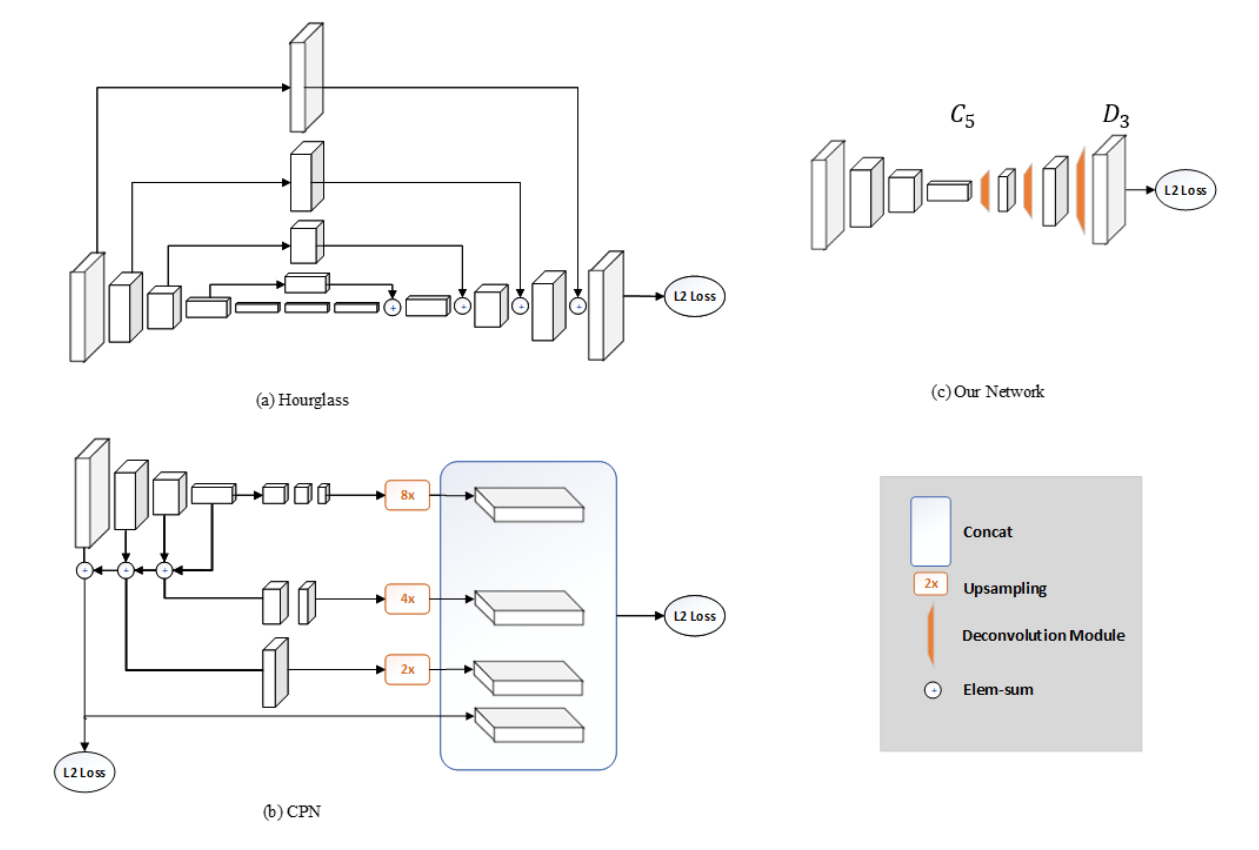
\includegraphics[scale=0.4]{figures/16.png}
	\caption{Hourglass网络结构\textsuperscript{\cite{p23}}}
	\label{fig:f16}
\end{figure}

沙漏结构的网络主要思路就是通过上采样将小尺寸的特征映射膨胀到原尺寸大小,然后与上一层的输入进行融合。在这个过程已经考虑了各个尺度的特征,所以沙漏网络具有良好效率,甚至可以无需经过复杂的多阶段训练,就能达到很高的精度。特别是对于小尺寸目标的分析,性能上要优于其他类型的网络结构。由于沙漏网络在输入与输出中只是改变特征图的深度,对于尺寸只是 2 倍的下采样或者上采样,所以在网络中应用沙漏网络也显得尤为方便。同时,在每个沙漏模块后都加以中间监督处理,加快了网络的收敛,提高了准确度。利用多个沙漏模型堆叠,在人体姿态估计任务中有十分优秀的表现,在 FLIC 和 MPII Human Pose 数据集上实现了2016年的 SOTA。

此外Chen等于2017年设计了一个级联金字塔残差模块(CPN, Cascaded  Pyramid Network)\textsuperscript{\cite{p24}}来进行多人人体姿态的估计。在 R-CNN 算法中,网络直接将网络的最后一层作为输出的预测层,在预测的阶段只使用最后一层作为所有特征的最后结果。这种方法具有明显的弊端,一般而言,随着网络的加深,特征图不断经过池化下采样处理,丢失的纹理特征越来越多;利用最后一层作为预测唯一特征映射,一方面对小尺度的目标没有很好的效果,甚至不能识别,另一方面浅层网络的纹理信息被大量地丢弃,训练出来的性能也受限。如果可以结合底层的特征映射图,这样的问题就可以得到一定程度的改良。

\begin{figure}[h]
	\centering
	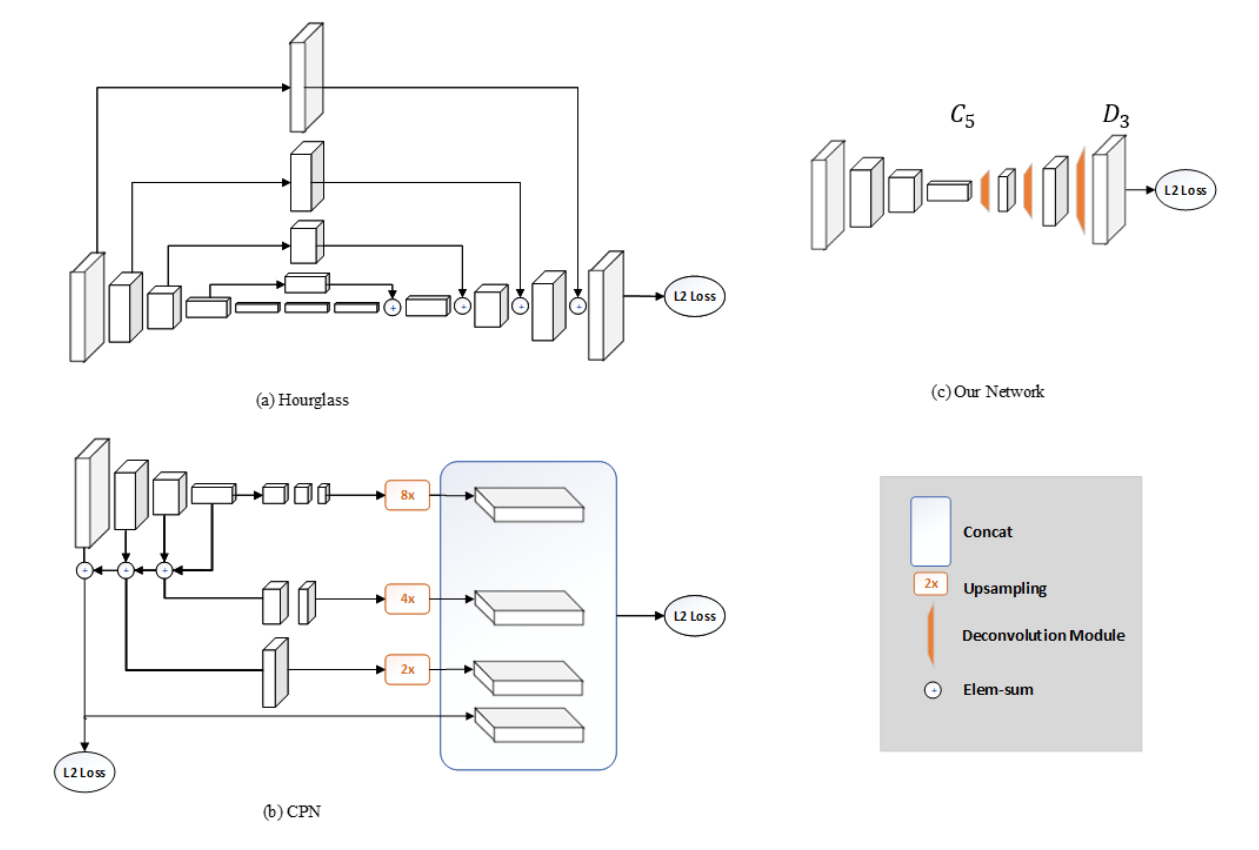
\includegraphics[scale=0.4]{figures/17.png}
	\caption{CPN网络结构\textsuperscript{\cite{p24}}}
	\label{fig:f17}
\end{figure}

金字塔网络模型旨在特征提取的时候,同时注重浅层网络的纹理特征和深层网络的语义特征,能够解决目标识别的尺度问题。思路是首先对于清晰可见、特征明确、易于检测关键点进行直接预测。而对于其他较为难以准确估计的关键点,如被遮挡的关节点、罕见姿态的部分部位、易于混淆的部位等,通过增大感受野并利用上下文信息的方式来进一步获得关键点位置。网络整体级联了两个金字塔结构的网络全局网络(GlobelNet)和优化网络(RefineNet)。其中,GolbalNet负责首先对所有关键点进行初步的检测,尤其对于特征较为明显的部位,如眼睛,胳膊等的关键点预测效果较好。RefineNet指的是对GolbalNet预测的结果进行修正的网络。主要修正身体部位中因为被遮挡,或者有复杂背景的误差较大的关键点。并在RefineNet的训练中使用了难例挖掘策略(OHEM, Online Hard Keypoints Mining),针对难以识别的关节点进行了加强训练。


\section{模型与方法}
所涉及的网络架构越来越复杂,在进行算法分析时的对照也愈加苦难,无法针对算法中的每一个细节设计进行细致准确且严谨的分析。故而本文希望在同时准确传局部信息和全局信息的同时构建更为简单的架构,采取了反卷积网络结构,利用热图进行二维人体姿态的估计。本文利用SimpleBaseline二维人体姿态估计模型\textsuperscript{\cite{p25}}将上采样与卷积参数利用反卷积层进行合并,而代替跳跃连接模块。

为了加速卷积神经网络的训练,用其中的像素值表示关键点在该位置存在的概率,能够提供更多的监督信息,而不仅仅是关节点坐标。如图\ref{fig:f18}所示,每个关节占据一个以目标关节位置为中心的二维高斯分布的热图通道。热图表示比坐标表示具有更强的鲁棒性,最近的研究大多基于热图表示。

\begin{figure}[h]
	\centering
	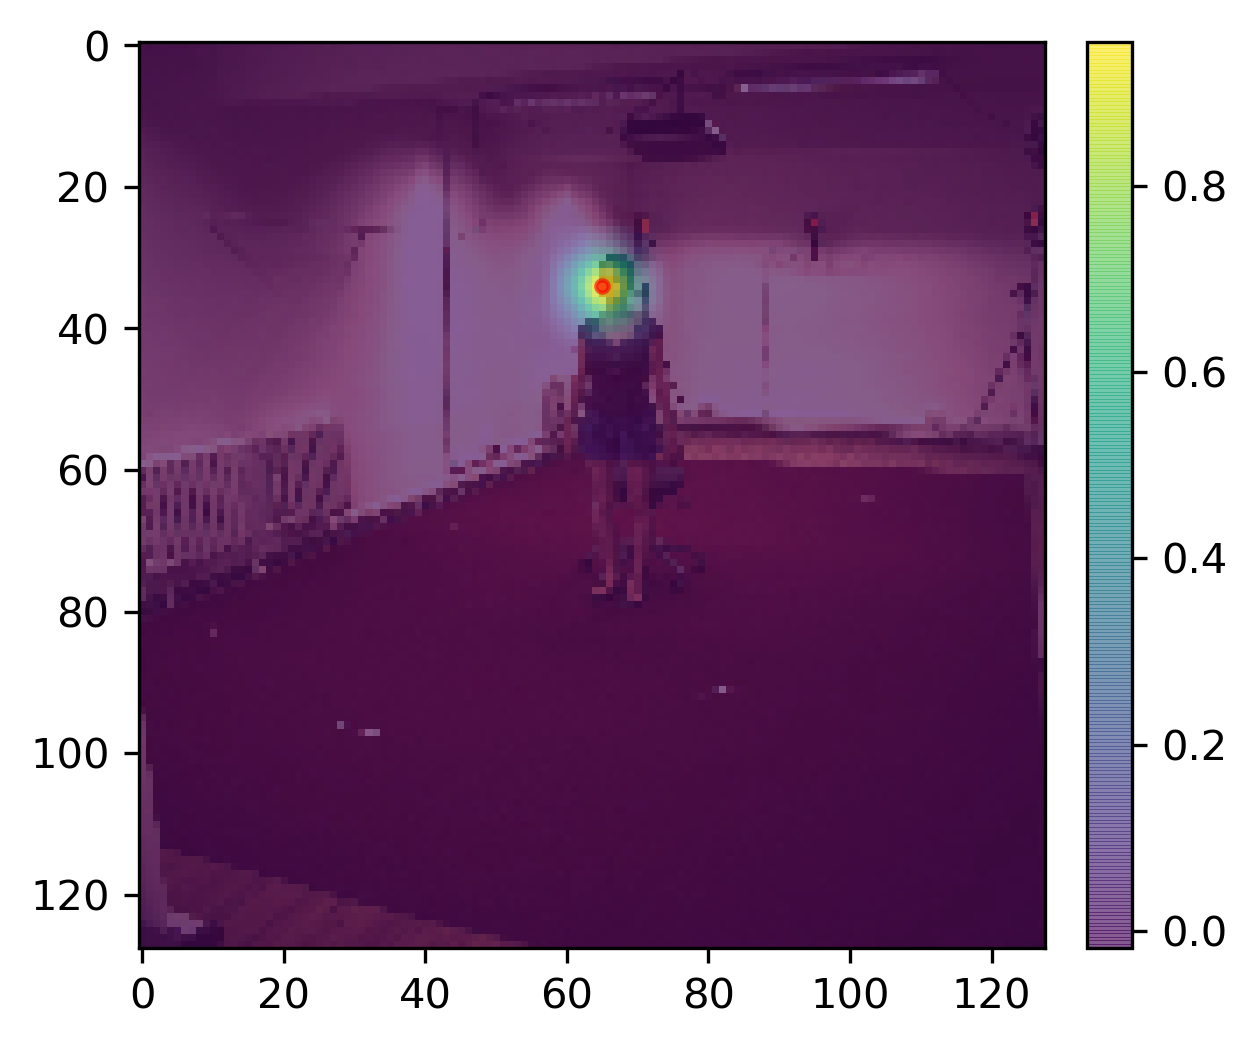
\includegraphics[scale=0.4]{figures/18.png}
	\caption{CPN网络结构}
	\label{fig:f18}
\end{figure}

本文的实验模型基于ResNet-50,设置Kernel-size为4,并在最后利用3个反卷积层生成64×48的热图。

\begin{figure}[h]
	\centering
	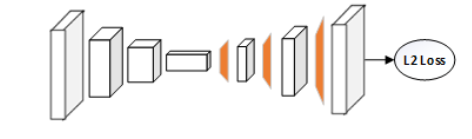
\includegraphics[scale=0.4]{figures/19.png}
	\caption{二维人体姿态估计网络模型\textsuperscript{\cite{p25}}}
	\label{fig:f19}
\end{figure}



\section{数据及实验}
\subsection{二维人体姿态数据集}{}

2D Pose 网络的训练和验证都需要使用一些公开的数据集,相对于三维人体姿态估计, 2D 人体姿态数据集较为丰富,这些数据集有较高质量图片的同时提供了其图像内人物的骨架二维坐标。这些数据集不仅提供了含有人体的图像数据,还提供了对应人体姿态的标注信息,方便训练自己的 2D 姿态估计网络,以下是一些常用公共数据集。

MPII 数据集,用来作为评价铰链式人体骨架的基准。该数据集一共大约有两万五千幅高质量图像,其中超过四万服含有人的高质量图是带有二维骨架坐标注释的,其骨架关键点数量为 16。这些图像来源于人类日常生活中,通过分类器收集完成,大概有 410 个不同的人类活动,且包含其对应的二维骨架坐标的标签;同时这些图像大多数都是从网络视频中提取,如 YouTube,所以还提供了很多没有标签信息的帧图像,这才一些方法的测试和训练中是十分有益的;同时其测试集含有对身体遮挡后的三维躯干以及方向的标注信息。

MSCOCO 数据集, 全称是 Miscrosoft COCO Dataset, 在检测数据集我们已经介绍过,所以此数据集十分大且用途也十分广泛,可以用来从事检测跟踪、分割、以及二维姿态估计等工作。这里我们只用到其人体二维骨架关键点信息,用来从事二维姿态估计,MSCOCO 数据集就含有人体骨架关节点信息部分而言,此部分包括超过 20 万张的各类源自网络的日常图片,所有图片一共有超过约 25万个不同人物做着各类动作,且为这些不同的人都标注了骨架坐标,其骨架关键点数量共有 18 个,所以我们可以看出该数据集的数据量是远超 MPII 的。

LSP 数据集,LSP 数据集全称是 Leeds Sports Pose Dataset,这个数据集数据量并不大,整体数据集的大约有两千个骨架标注信息的图像,数据集中的这些图像大多都是是从 Filcker 获取的\textsuperscript{\cite{p17}},其主要针对运动目标人物任务相关的数据集,所以所有图片要求不仅要包含人体骨架标注信息,还要求包含各类运动的类别标签,方便区分不同运动类别,其人体骨架关键点数量为 14。

AI Challenge 数据集, 其一共包含了大约 27 万幅图,同时含有人体骨架标注信息,一般而言,一般将其中 21 万幅图用来训练网络,验证集和测试集数据分别为三万幅图,其人体骨架关键点数量是 14 个,包含三十八万个不同人的数据集。

本文的工作主要采用COCOtrain2017数据集,包含57k张图像和150k个人体实例,并在test-dev2017数据集上进行测试和评价。

\subsection{实验结果}{}
OKS(object keypoint similarity)是目前常用的人体骨骼关键点检测算法的评价指标,这个指标启发于目标检测中的IoU指标,可以衡量估计的关节点位置与真实标签的相似度。

二维人体姿态估计所采用的评价指标为平均精确度(AP, Average Precision)。对目标进行关键点检测后会获得一组关键点(DT),最后会计算出GT与DT的相似度oks为一个标量,然后人为的给定一个阈值T,然后可以通过所有图片的oks计算AP,本实验中,设置T为10。

训练过程中的准确率Accuracy曲线如图3-5,其中准确率为PCK(Percentage of Correct Keypoints),描述估计正确的关节点的占比。

本文将数据集中每个目标按照bounding box裁剪为分辨率为256:192的图像,并采用±30%的缩放,±40°的旋转和翻转做数据增强。基本学习率为0.001,在90epoch后下降为0.0001,在120epoch后下降为0.00001,利用深度为50层的ResNet进行训练,训练及测试结果如下。

\begin{figure}[h]
	\centering
	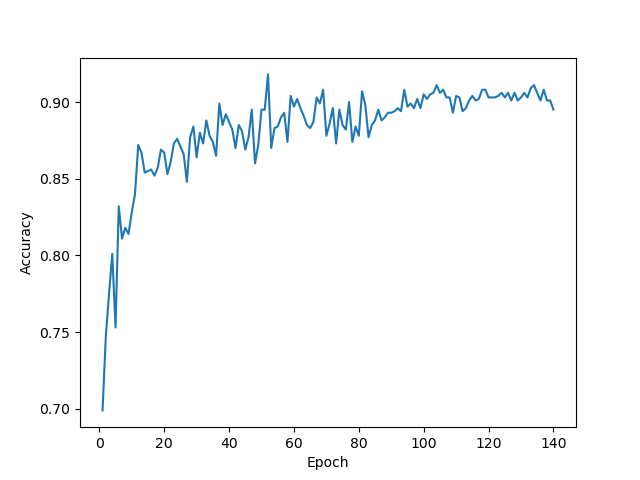
\includegraphics[scale=0.4]{figures/20.png}
	\caption{二维人体姿态估计模型Accuracy-Epoch曲线}
	\label{fig:f20}
\end{figure}

\begin{figure}[h]
	\centering
	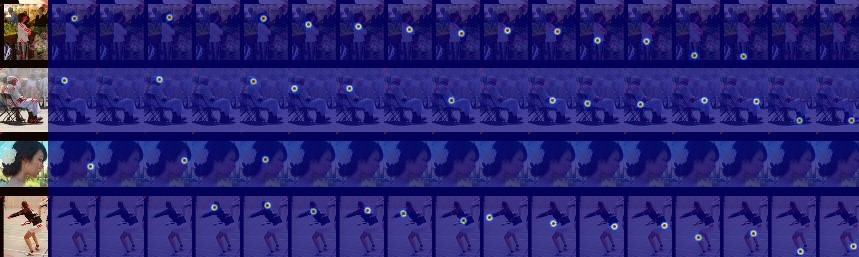
\includegraphics[scale=0.4]{figures/21.jpg}
	\caption{coco部分测试数据关节点真实标注}
	\label{fig:f21}
\end{figure}

\begin{figure}[h]
	\centering
	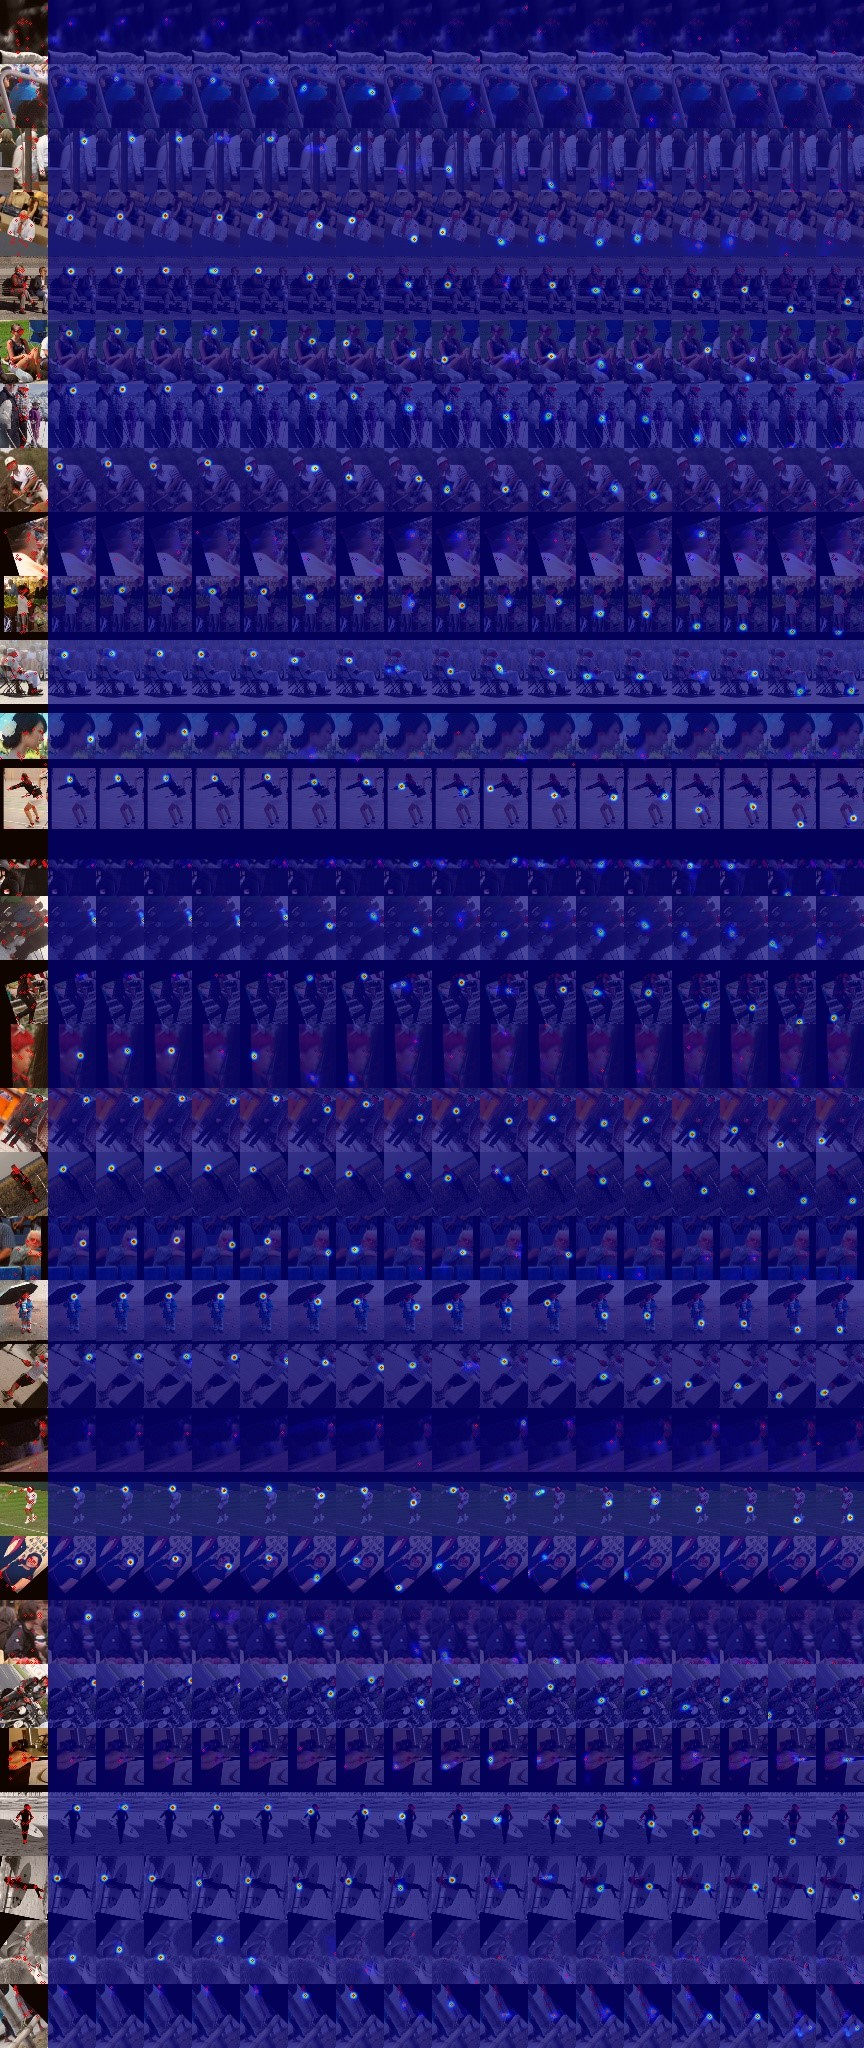
\includegraphics[scale=0.4]{figures/22.jpg}
	\caption{coco部分测试数据关节点估计结果}
	\label{fig:f22}
\end{figure}

\begin{table}[h]
    \caption{\label{tab:t1}二维人体姿态估计模型测试结果}
    \centering
    \begin{tabular}{c c c c c c c c c c c}
        \toprule
        Index	   & AP	    & Ap.5	    & AP.75	    & APm	    & APl	    & AR	    & AR.5	    & AR.75	    & ARm	    & ARl   \\
        \midrule
        Results   & 0.712	& 0.914	    & 0.796     & 0.791	    & 0.685	    & 0.759	    & 0.745	    & 0.923	    & 0.813	    & 0.712   \\
        \bottomrule
    \end{tabular}
\end{table}

\begin{table}[h]
    \caption{\label{tab:t2}各二维人体姿态估计模型AP对比(Input Size=256×192, no OHKM)}
    \centering
    \begin{tabular}{c c}
        \toprule
        Method	   & AP	 \\
        \midrule
        Hourglass(8-stage)	& 0.669 \\
        CPN(ResNet-50)	    & 0.686 \\
        ours(ResNet-50)	    & 0.712 \\
        \bottomrule
    \end{tabular}
\end{table}